\documentclass{article}
%\VignetteIndexEntry{Using SemDist}
%\newcommand{\tab}[1]{\hspace{.2\textwidth}\rlap{#1}}
\usepackage{amsmath}
\usepackage[hidelinks]{hyperref}
\usepackage{cleveref}
\usepackage{natbib}
\usepackage{url}

\title{An Introduction to SemDist}
\usepackage{Sweave}
\begin{document}
\Sconcordance{concordance:introduction.tex:introduction.rnw:%
1 10 1 1 0 142 1 1 2 1 0 1 1 3 0 1 5 10 1 1 3 2 0 1 1 7 0 1 5 3 0 1 1 3 %
0 1 2 4 1 1 5 3 0 1 2 1 0 1 3 5 0 1 2 3 1 1 4 6 0 1 2 19 1 1 4 3 0 1 2 %
1 0 2 1 12 0 1 2 6 1 1 2 1 0 2 1 3 0 1 2 7 1 1 3 2 0 1 1 1 5 6 0 1 2 9 %
1 1 2 1 0 2 1 4 0 1 2 7 1 1 4 3 0 1 1 6 0 1 2 9 1 1 3 2 0 2 1 4 0 1 2 7 %
1}


\begin{center}

{\Large\bf An Introduction to the SemDist package\\
Version 0.99.0\\
\vspace*{0.5cm}
%Ian Gonzalez\\
%\vspace*{0.5cm}

%%%%%%%%%%%%%%%%%%%%%%%%%%%%%
% Add more title
%%%%%%%%%%%%%%%%%%%%%%%%%%%%%

}

\end{center}

\tableofcontents
\clearpage
%%%%%%%%%%%%%%%%%%%%%%%%%%%%%%%%%%%%%%%%%%%%%%%%%%%%%%%%%%%%%%%%%%%%%%%%%%%%%%%%%%%%%%%
%%%%%%%%%%%%%%%%%%%%%%%%%%%%%%%%%%%%%%%%%%%%%%%%%%%%%%%%%%%%%%%%%%%%%%%%%%%%%%%%%%%%%%%
\section{Overview and Background}
%%%%%%%%%%%%%%%%%%%%%%%%%%%%%%%%%%%%%%%%%%%%%%%%%%%%%%%%%%%%%%%%%%%%%%%%%%%%%%%%%%%%%%%
%%%%%%%%%%%%%%%%%%%%%%%%%%%%%%%%%%%%%%%%%%%%%%%%%%%%%%%%%%%%%%%%%%%%%%%%%%%%%%%%%%%%%%%

\hspace{0.5cm} The methods in this package assess the performance of a predictor of multi-label annotations, such that labels are drawn from an ontology structured as a directed acyclic graph (DAG).  The package was designed to work specifically with the Gene Ontology (GO) \citep{Ashburner2000}, but functionality has been embedded that will allow users to define their own ontology in addition to probability distributions associated with ``entities" in the given ontology.  The basic inputs to the package are sets of true GO terms associated with each data-point (be it a gene or protein), and sets of predicted annotations with associated confidence values in the interval $[0,1]$. The SemDist package facilitates the calculation of several statistics relating to the performance of a given predictor, all of which utilize the concept of information accretion as their foundation \citep{Clark2013}.

%%%%%%%%%%%%%%%%%%%%%%%%%%%%%%%%%%%%%%%%%%%%%%%%%%%%%%%%%%%%%%%%%%%%%%%%%%%%%%%%%%%%%%%
%%%%%%%%%%%%%%%%%%%%%%%%%%%%%%%%%%%%%%%%%%%%%%%%%%%%%%%%%%%%%%%%%%%%%%%%%%%%%%%%%%%%%%%
\subsection{Metric definitions}
%%%%%%%%%%%%%%%%%%%%%%%%%%%%%%%%%%%%%%%%%%%%%%%%%%%%%%%%%%%%%%%%%%%%%%%%%%%%%%%%%%%%%%%
%%%%%%%%%%%%%%%%%%%%%%%%%%%%%%%%%%%%%%%%%%%%%%%%%%%%%%%%%%%%%%%%%%%%%%%%%%%%%%%%%%%%%%%

Briefly, the concept of information accretion arises from interpreting an ontology as a Bayesian network.  In this framework,  the joint probability of a set of ``states" in the network (in this case true or false values associated to terms) is calculated by considering the conditional probability of each individual variable given its parents.

Very simply, information accretion is calculated by considering the conditional probability of a term given its parents,
\begin{equation}
ia(v)= \frac{1}{Pr(v|\mathcal{P}(v))},
\label{eq:IA}
\end{equation}
where $\mathcal{P}(v)$ refers to the parents of vertex $v$. Using information accretion the information content of a set of terms $T$, representing a consistent subgraph from the overall DAG, can then be calculated as

\begin{equation}
i(T)  = \underset{v\in T}{\sum}ia(v).
\end{equation}

Although the SemDist package calculates several information accretion based metrics users might be more familiar with such as precision, recall, and specificity; the hallmarks of the package are the previously introduced metrics misinformation and remaining uncertainty.


Specifically, the \emph{remaining uncertainty} about a protein's true annotation corresponds to the information about the protein that is not yet provided by the graph $P$. More formally, we express remaining uncertainty ($ru$) as

\begin{equation}
ru(T,P)=\underset{v\in T\setminus P}{\sum}ia(v),
\label{eq:ruSIMP}
\end{equation}


\noindent which is simply the total information content of the nodes in the ontology that are contained in true annotation $T$ but not in the predicted annotation $P$. Note that, in a slight abuse of notation, we apply set operations to graphs to manipulate only the vertices of these graphs.


The \emph{misinformation} introduced by the classifier corresponds to the total information content of the nodes along incorrect paths in the prediction graph $P$. More formally, misinformation is expressed as

\begin{equation}
mi(T,P)=\underset{v\in P\setminus T}{\sum}ia(v),
\label{eq:miSIMP}
\end{equation}

\noindent which quantifies how misleading a predicted annotation is. 

For a more thorough, formal treatment of the theory behind these metrics, see \citet{Clark2013} and \citet{Clark2014Information}.

\Cref{eq:ruSIMP,eq:miSIMP} illustrate calculating remaining uncertainty and misinformation in a very simple case where there is a single data point and no probabilities associated with each predicted term. SemDist performs calculations by averaging over the entire set of proteins used in evaluation, i.e.

\begin{equation}
ru(\tau)=\frac{1}{n}\sum_{i=1}^{n}ru(T_{i},P_{i}(\tau))
\label{eq:average_ru}
\end{equation}


\noindent and

\begin{equation}
mi(\tau)=\frac{1}{n}\sum_{i=1}^{n}mi(T_{i},P_{i}(\tau))
\label{eq:average_mi}
\end{equation}


\noindent where $n$ is the number of proteins in the data set, $T_{i}$ is the true set of terms for protein $x_{i}$, and $P_{i}(\tau)$ is the set of predicted terms for protein $x_{i}$ given decision threshold $\tau$. 

Once the set of terms with scores greater than or equal to $\tau$ is determined, the set $P_{i}(\tau)$ is composed of the unique union of the ancestors of all predicted terms. As the decision threshold is moved from its minimum ($0$) to its maximum value ($1$), the pairs of $(ru(\tau),mi(\tau))$ will result in a curve in 2D space. We refer to such a curve using $(ru(\tau),mi(\tau))_{\tau}$. Removing the normalizing constant ($\frac{1}{n}$) from the above equations would result in the total remaining uncertainty and misinformation associated with a database of proteins and a set of predictions.

Finally, to provide a single performance measure which can be used to rank and evaluate protein function prediction algorithms, we introduced \emph{semantic distance} as the minimum distance from the origin to the curve $(ru(\tau),mi(\tau))_{\tau}$. More formally, the semantic distance $S_{k}$ is defined as

\begin{equation}
S_{k}=\underset{\tau}{\min}(ru^{k}(\tau)+mi^{k}(\tau))^{\frac{1}{k}},
\label{eq:semantic_distance}
\end{equation}

\noindent where $k$ is a positive integer. Setting $k=2$ results in the minimum Euclidean distance on the curve from the origin.
 
We have also generalize the definitions of precision and recall into their information formulation. Here, precision and recall can be expressed as

\begin{equation}
pr(T,P(\tau))=\frac{\underset{v\in T\cap P(\tau)}{\sum}ia(v)}{\underset{v\in P(\tau)}{\sum}ia(v)}
\label{eq:precision}
\end{equation}

\noindent and

\begin{equation}
rc(T,P(\tau))=\frac{\underset{v\in T\cap P(\tau)}{\sum}ia(v)}{\underset{v\in T}{\sum}ia(v)}.
\label{eq:recall}
\end{equation}

Precision $pr(\tau)$ and recall $rc(\tau)$ can then be calculated as averages over the database of proteins for each threshold $\tau$, as in Equations \Cref{eq:average_ru,eq:average_mi}.

Our framework also facilitates calculating specificity

\begin{equation}
%wsp(T,P(\tau))=\frac{ \underset{v\in \stcomp{T} \cap \stcomp{P} }{\sum}ia(v)}{\underset{v\in \stcomp{T}}{\sum}ia(v)}
sp(T,P(\tau))=\frac{\underset{v\in T^{\bf{c}} \cap P^{\bf{c}}(\tau)}{\sum}ia(v)}{\underset{v\in T^{\bf{c}}}{\sum}ia(v)}
\label{eq:weighted_specificity}
\end{equation}
where $T^{\bf{c}}$ represents the complement of set $T$. Combining specificity and recall (sensitivity) facilitate plotting an ROC curve and calculating AUROC.

Finally, we facilitate the calculation of semantic similarity,

\begin{equation}
ss(T,P(\tau))=\underset{v\in T\cap P(\tau)}{\sum{ia(v)}},
\label{eq:semsem}
\end{equation}
a formulation similar to that defined by \citet{Resnik1995} and \citet{Lord2003}.

This package allows for straightforward calculation of these metrics. It provides a set of methods for calculating the information accretion for each term in a given ontology in addition to providing pre-calculated values for a set of organisms.
%%%%%%%%%%%%%%%%%%%%%%%%%%%%%%%%%%%%%%%%%%%%%%%%%%%%%%%%%%%%%%%%%%%%%%%%%%%%%%%%%%%%%%%
%%%%%%%%%%%%%%%%%%%%%%%%%%%%%%%%%%%%%%%%%%%%%%%%%%%%%%%%%%%%%%%%%%%%%%%%%%%%%%%%%%%%%%%
\section{Installation and Requirements}
%%%%%%%%%%%%%%%%%%%%%%%%%%%%%%%%%%%%%%%%%%%%%%%%%%%%%%%%%%%%%%%%%%%%%%%%%%%%%%%%%%%%%%%
%%%%%%%%%%%%%%%%%%%%%%%%%%%%%%%%%%%%%%%%%%%%%%%%%%%%%%%%%%%%%%%%%%%%%%%%%%%%%%%%%%%%%%%

Install the SemDist package on your version of R with the biocLite and library functions. The package requires R version 2.10.0 or greater and Bioconductor version 2.14 or greater. The annotate, AnnotationDbi, and GO.db packages are also required for functionality.
\begin{Schunk}
\begin{Sinput}
> biocLite("SemDist")
> library(SemDist)
\end{Sinput}
\end{Schunk}

%%%%%%%%%%%%%%%%%%%%%%%%%%%%%%%%%%%%%%%%%%%%%%%%%%%%%%%%%%%%%%%%%%%%%%%%%%%%%%%%%%%%%%%
%%%%%%%%%%%%%%%%%%%%%%%%%%%%%%%%%%%%%%%%%%%%%%%%%%%%%%%%%%%%%%%%%%%%%%%%%%%%%%%%%%%%%%%
\section{Calculating information accretion values}
%%%%%%%%%%%%%%%%%%%%%%%%%%%%%%%%%%%%%%%%%%%%%%%%%%%%%%%%%%%%%%%%%%%%%%%%%%%%%%%%%%%%%%%
%%%%%%%%%%%%%%%%%%%%%%%%%%%%%%%%%%%%%%%%%%%%%%%%%%%%%%%%%%%%%%%%%%%%%%%%%%%%%%%%%%%%%%%

The simplest way to use SemDist is to use one of the provided data sets containing information accretion values. Information accretion values were pre-calculated for each organism using Bioconductor AnnotationData Packages \citep{Anno}. These pre-calculated values can be found in the \path{data/} directory of the SemDist package. (Note that in addition, all other test files used in the following examples can be accessed by the user in the \path{extdata/} directory). Calculations were performed using only annotations supported by experimental evidence codes (EXP, IDA, IPI, IMP, IGI, IEP, TAS, IC). 

Information accretion values can be recalculated by the user or calculated using different evidence codes using the \texttt{computeIA} function.

\begin{Schunk}
\begin{Sinput}
> # Examine built-in IA data
> data("Info_Accretion_mouse_CC", package="SemDist")
> head(IAccr)
\end{Sinput}
\begin{Soutput}
GO:0000015 GO:0005886 GO:0000109 GO:0000110 GO:0000111 GO:0000112 
4.56985561 0.00849539 6.11173759 2.70043972 3.70043972 3.70043972 
\end{Soutput}
\end{Schunk}
\begin{Schunk}
\begin{Sinput}
> # Calculate IA, specify evidence codes
> # Requires downloading annotation data package
> biocLite("org.Hs.eg.db")
> IAccr <- computeIA("MF", "human", evcodes=c("EXP", "IC"))
\end{Sinput}
\end{Schunk}

Users can define their own ontology and annotations.  The \texttt{computeIA} function can then calculate information accretion for each term, or entity, in the custom ontology according to \Cref{eq:IA}.

Ontologies should be specified using a tab-delimited file indicating every parent-child relationship in the ontology; with the first column designating the parent name and the second column identifying the child name. The annotations file should have the same format as the true annotations file used above where annotations represent terms drawn from the specified ontology.  

\begin{Schunk}
\begin{Sinput}
> # Calculate IA, specify ontology and annotations
> ontfile <- system.file("extdata", "mfo_ontology.txt",
+                         package="SemDist")
> annotations <- system.file("extdata", "MFO_LABELS_TEST.txt", 
+                             package="SemDist")
> IAccr <- computeIA("my", "values", specify.ont=TRUE, 
+                 myont=ontfile, specify.annotations=TRUE, 
+                 annotfile=annotations)
\end{Sinput}
\end{Schunk}


It is also possible to specify your own ontology and use Bioconductor AnnotationData annotations, although it should be pointed out that using a version of the ontology other than that associated with the AnnotationData annotations may result in terms not being found. 

\begin{Schunk}
\begin{Sinput}
> # Calculate IA, specify ontology
> IAccr <- computeIA("MF", "human", specify.ont=TRUE,
+          myont=ontfile, specify.annotations=FALSE)
\end{Sinput}
\end{Schunk}


When the ontology is specified but annotations are not, annotations are taken from the specified organism. (Note that this may require the installation of databases not provided in the package). The recommended method is to specify both, as is the case in the second example. 

The information accretion data generated in this way can be used in the \texttt{findRUMI} and \texttt{RUMIcurve} functions (which will be discussed below).

%%%%%%%%%%%%%%%%%%%%%%%%%%%%%%%%%%%%%%%%%%%%%%%%%%%%%%%%%%%%%%%%%%%%%%%%%%%%%%%%%%%%%%%
%%%%%%%%%%%%%%%%%%%%%%%%%%%%%%%%%%%%%%%%%%%%%%%%%%%%%%%%%%%%%%%%%%%%%%%%%%%%%%%%%%%%%%%
\section{Getting Started with RU-MI Calculations}
%%%%%%%%%%%%%%%%%%%%%%%%%%%%%%%%%%%%%%%%%%%%%%%%%%%%%%%%%%%%%%%%%%%%%%%%%%%%%%%%%%%%%%%
%%%%%%%%%%%%%%%%%%%%%%%%%%%%%%%%%%%%%%%%%%%%%%%%%%%%%%%%%%%%%%%%%%%%%%%%%%%%%%%%%%%%%%%

Before any of the evaluation metrics in this package can be utilized, two user-provided data sets are needed in the working directory:
\begin{enumerate}
\item A file containing true annotations of the protein sequences being looked at.
\item A file containing the annotations predicted by the function predictor along with a $[0-1]$ probability assigned to each annotation.
\end{enumerate}

These files should take the form of tab-delineated text, with the first column being sequence identifiers, the second column being GO identifiers (of the form "GO:0005615"), and the third column (in the case of the prediction file) being a valid number in the interval $[0,1]$.

\begin{Schunk}
\begin{Sinput}
> # Sample true, prediction files included with SemDist:
> truefile <- system.file("extdata", "MFO_LABELS_TEST.txt", 
+                         package="SemDist")
> predfile <- system.file("extdata", "MFO_PREDS_TEST.txt", 
+                         package="SemDist")
> predictions <- read.table(predfile, colClasses = "character")
> head(predictions)
\end{Sinput}
\begin{Soutput}
          V1         V2    V3
1 INO4_YEAST GO:0003674 0.464
2 INO4_YEAST GO:0030528 0.464
3 INO4_YEAST GO:0016564 0.441
4 INO4_YEAST GO:0016563 0.464
5 INO4_YEAST GO:0030234 0.400
6 INO4_YEAST GO:0060589 0.400
\end{Soutput}
\end{Schunk}


Given these basic data sets, remaining uncertainty and misinformation can be calculated according to \Cref{eq:ruSIMP} and \Cref{eq:miSIMP} using the \texttt{findRUMI} function in addition to the package's built in data sets. 


As a simple example we show how one can calculate remaining uncertainty and misinformation for a single threshold ($\tau =0.75$),

\begin{Schunk}
\begin{Sinput}
> rumiTable <- findRUMI("MF", "human", 0.75, truefile, predfile)
> avgRU <- mean(rumiTable$RU)
> avgMI <- mean(rumiTable$MI)
\end{Sinput}
\end{Schunk}

where information accretion data from the molecular function portion of the ontology terms annotating human sequences were used (denoted \texttt{"MF"} and \texttt{"human"} in the function call). 


The returned \texttt{rumiTable} variable should contains a data frame with the remaining uncertainty values for each sequence in the first column and the corresponding misinformation values in the second column. Single-number metrics can be obtained by averaging across the entire set.

As mentioned in the above section, user-created IA variables from \texttt{computeIA} output can be used to specify the information accretion values used in the calculation of \texttt{RU} and \texttt{MI} via the \texttt{IAccr} argument:

\begin{Schunk}
\begin{Sinput}
> # A sample IA file that comes with the SemDist package.
> myIA <- system.file("extdata", "myIA.rda", package="SemDist")
> load(myIA)
> # "MF" and "human" are present only for naming purposes
> # since IA is taken from myIA.rda
> rumiTable <- findRUMI("MF", "human", 0.75, truefile, predfile, 
+                         IAccr = IA)
\end{Sinput}
\end{Schunk}

%%%%%%%%%%%%%%%%%%%%%%%%%%%%%%%%%%%%%%%%%%%%%%%%%%%%%%%%%%%%%%%%%%%%%%%%%%%%%%%%%%%%%%%
%%%%%%%%%%%%%%%%%%%%%%%%%%%%%%%%%%%%%%%%%%%%%%%%%%%%%%%%%%%%%%%%%%%%%%%%%%%%%%%%%%%%%%%
\section{Creating a RU-MI Curve}
%%%%%%%%%%%%%%%%%%%%%%%%%%%%%%%%%%%%%%%%%%%%%%%%%%%%%%%%%%%%%%%%%%%%%%%%%%%%%%%%%%%%%%%
%%%%%%%%%%%%%%%%%%%%%%%%%%%%%%%%%%%%%%%%%%%%%%%%%%%%%%%%%%%%%%%%%%%%%%%%%%%%%%%%%%%%%%%


The average values of remaining uncertainty and misinformation across multiple thresholds in the interval $[0,1]$ as specified by \Cref{eq:average_ru,eq:average_mi} can be calculated. Using the same true/prediction files and specifying a set increment of $0.05$ which $\tau$ is increased

\begin{Schunk}
\begin{Sinput}
> avgRUMIvals <- RUMIcurve("MF", "human", 0.05, truefile, predfile)
> firstset <- avgRUMIvals[[1]]
> plot(firstset$RU, firstset$MI)
\end{Sinput}
\end{Schunk}
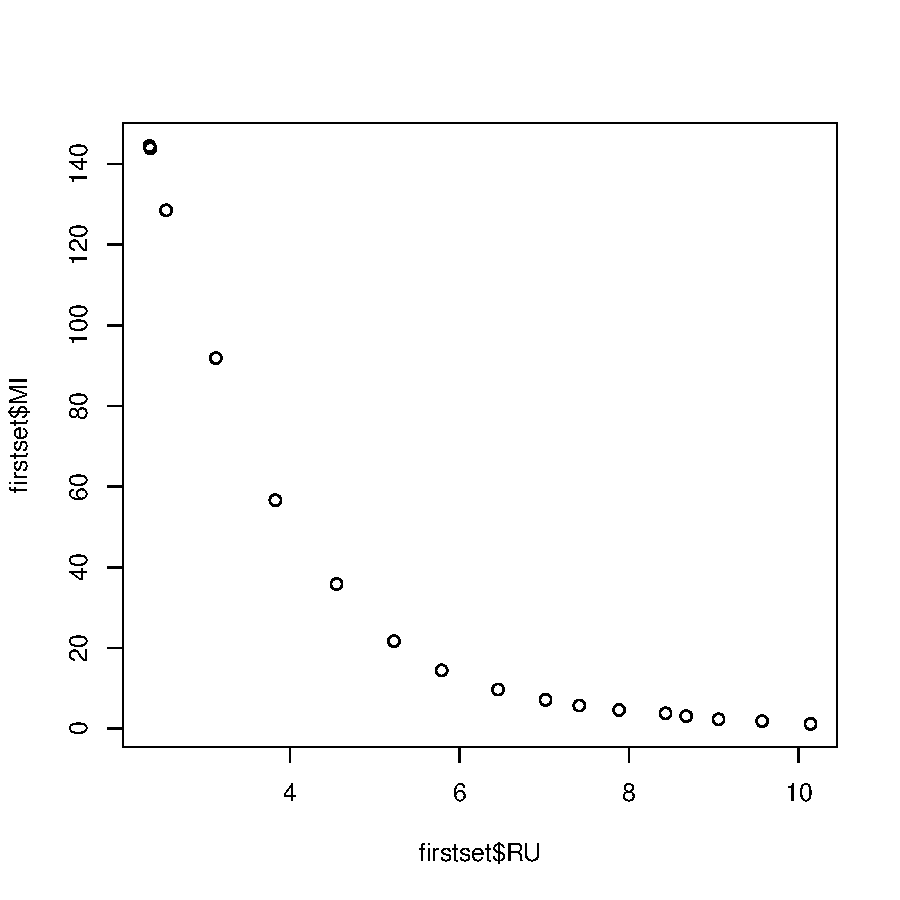
\includegraphics{introduction-010}


The \texttt{RUMIcurve} function will accept multiple prediction files (as a character vector) as input, and actually returns a list containing the values calculated for each set of predictions; hence the need for indexing into the first element to get the curve data. The \texttt{firstset} variable contains a data frame with the average RU and MI values for each threshold the function calculated for. In this case, the increment was set to 0.05.

The plot visualizes how remaining uncertainty and misinformation change as the decision threshold is varried. If multiple predictions are input they can be quickly compared.

Semantic distance can be obtained in a straightforward manner from the points in the RU-MI curve according to \Cref{eq:semantic_distance}:

\begin{Schunk}
\begin{Sinput}
> # Minimize distance from origin over all points in RUMI curve:
> 
> semdist <- min(sqrt(firstset$MI^2 + firstset$RU^2))
> semdist
\end{Sinput}
\begin{Soutput}
[1] 9.12004
\end{Soutput}
\end{Schunk}


%%%%%%%%%%%%%%%%%%%%%%%%%%%%%%%%%%%%%%%%%%%%%%%%%%%%%%%%%%%%%%%%%%%%%%%%%%%%%%%%%%%%%%%
%%%%%%%%%%%%%%%%%%%%%%%%%%%%%%%%%%%%%%%%%%%%%%%%%%%%%%%%%%%%%%%%%%%%%%%%%%%%%%%%%%%%%%%
\section{Additional metrics}
%%%%%%%%%%%%%%%%%%%%%%%%%%%%%%%%%%%%%%%%%%%%%%%%%%%%%%%%%%%%%%%%%%%%%%%%%%%%%%%%%%%%%%%
%%%%%%%%%%%%%%%%%%%%%%%%%%%%%%%%%%%%%%%%%%%%%%%%%%%%%%%%%%%%%%%%%%%%%%%%%%%%%%%%%%%%%%%

Related metrics can also be output by the \texttt{RUMIcurve} function. The data frames that are returned also contain an \texttt{"SS"} column which contains the semantic similarity for a given threshold calculated as specified by \Cref{eq:semsem}. Setting the boolean parameter \texttt{add.prec.rec} to TRUE will cause precision, recall, and specificity values to be included as well. Doing the same for \texttt{add.weighted} will output weighted remaining uncertainty, weighted misinformation, and weighted semantic similarity. The weighted metrics assign a weight to each RU or MI value for all the sequences based on how much of the total information accretion that sequence accounts. See \Cref{eq:precision}, \Cref{eq:recall}, and \Cref{eq:weighted_specificity} for the formal definitions of these calculations.

\begin{Schunk}
\begin{Sinput}
> rumiout <- RUMIcurve("MF", "human", 0.05, truefile, predfile,
+                      add.prec.rec=TRUE, add.weighted=TRUE)
> firstset <- rumiout[[1]]
> plot(firstset$WRU, firstset$WMI)
\end{Sinput}
\end{Schunk}
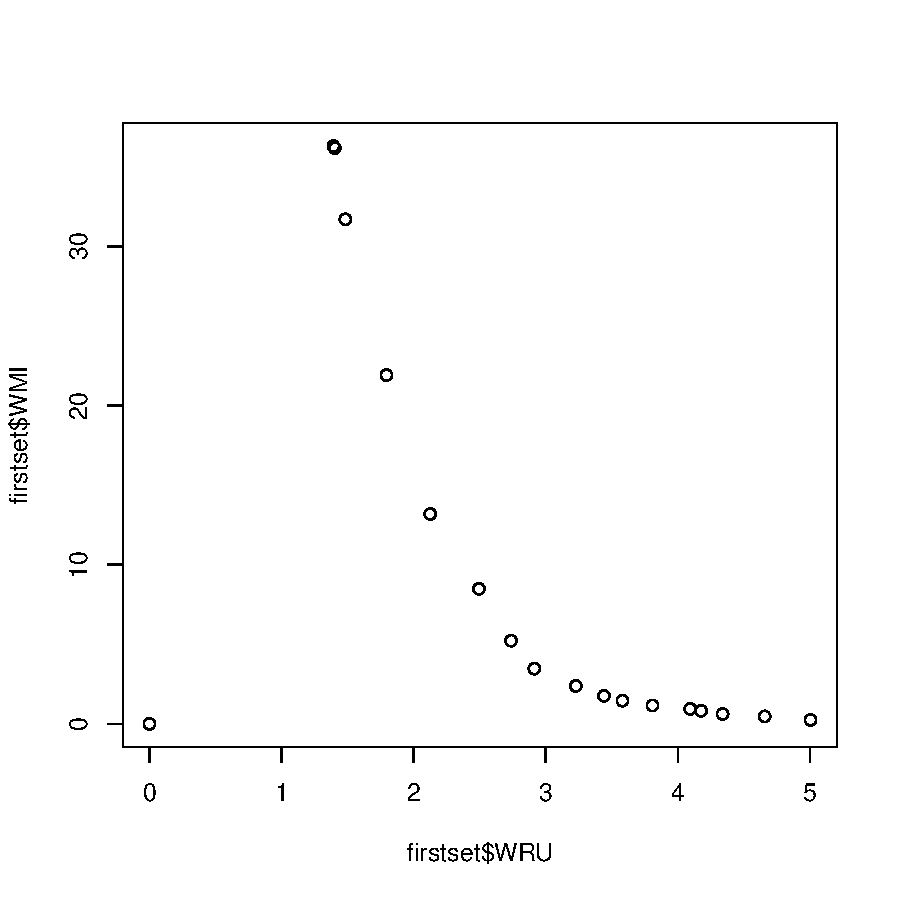
\includegraphics{introduction-012}

\section{Acknowledgments}
The code in the SemDist package was based in part on the source code of the GOSemSim package \citep{Yu2010}.
\bibliographystyle{plainnat}
\bibliography{refdbshort}


\end{document}
